\documentclass{article}
\usepackage[utf8]{inputenc} % Handle UTF-8 encoding
\usepackage{amsmath, amssymb, tikz, geometry, multicol}
\usepackage{pgfplots} % Added for plotting graphs
\pgfplotsset{compat=1.17}
\geometry{margin=0.25in}
\begin{document}

\begin{multicols}{2}

\section*{Polynomials Cheat Sheet}

\subsection*{Factoring Quadratics}

\subsubsection*{Standard Form}

A quadratic equation in standard form:

\[
ax^2 + bx + c = 0
\]

\subsubsection*{Quadratic Formula}

The solutions (roots) of the quadratic equation are given by the quadratic formula:

\[
x = \frac{-b \pm \sqrt{b^2 - 4ac}}{2a}
\]

\textbf{Discriminant}:

\[
D = b^2 - 4ac
\]

- If \( D > 0 \), there are two real and distinct roots.
- If \( D = 0 \), there is one real root (a repeated root).
- If \( D < 0 \), there are two complex conjugate roots.

\textbf{Example}:

Solve \( x^2 - 4x + 3 = 0 \).

Compute the discriminant:

\[
D = (-4)^2 - 4(1)(3) = 16 - 12 = 4
\]

Since \( D > 0 \), there are two real roots.

\[
x = \frac{-(-4) \pm \sqrt{4}}{2(1)} = \frac{4 \pm 2}{2}
\]

Thus, \( x = 3 \) or \( x = 1 \).

\subsubsection*{Difference and Sum of Squares}

- \textbf{Difference of Squares}:

\[
a^2 - b^2 = (a + b)(a - b)
\]

\textbf{Example}:

\[
x^2 - 9 = (x + 3)(x - 3)
\]

- \textbf{Sum of Squares}:

Note: \( a^2 + b^2 \) cannot be factored over real numbers.

\subsubsection*{Perfect Square Trinomials}

- \textbf{Perfect Square Trinomial}:

\[
a^2 \pm 2ab + b^2 = (a \pm b)^2
\]

\textbf{Examples}:

\[
x^2 + 6x + 9 = (x + 3)^2
\]

\[
x^2 - 10x + 25 = (x - 5)^2
\]

\subsubsection*{Factoring Quadratics with Leading Coefficient}

When \( a \neq 1 \), factor using methods such as:

- \textbf{Trial and Error}
- \textbf{AC Method}

\textbf{AC Method Steps}:

1. Multiply \( a \) and \( c \) to get \( ac \).
2. Find two numbers \( m \) and \( n \) such that \( m \times n = ac \) and \( m + n = b \).
3. Rewrite the quadratic as \( ax^2 + mx + nx + c \).
4. Factor by grouping.

\textbf{Example}:

Factor \( 2x^2 + 7x + 3 \).

1. \( a = 2 \), \( b = 7 \), \( c = 3 \).
2. \( ac = 2 \times 3 = 6 \).
3. Find \( m = 6 \), \( n = 1 \) (since \( 6 \times 1 = 6 \) and \( 6 + 1 = 7 \)).
4. Rewrite: \( 2x^2 + 6x + x + 3 \).
5. Factor by grouping:

\[
\begin{aligned}
& (2x^2 + 6x) + (x + 3) \\
& 2x(x + 3) + 1(x + 3) \\
& (2x + 1)(x + 3)
\end{aligned}
\]

\subsubsection*{Factoring by Grouping}

Used when there are four terms.

\textbf{Example}:

Factor \( x^3 + 3x^2 + 2x + 6 \).

1. Group terms: \( (x^3 + 3x^2) + (2x + 6) \).
2. Factor out GCF from each group:

\[
\begin{aligned}
& x^2(x + 3) + 2(x + 3) \\
& (x^2 + 2)(x + 3)
\end{aligned}
\]

\subsubsection*{Completing the Square}

Used to solve quadratics or rewrite them in vertex form.

\textbf{Steps}:

1. Ensure \( a = 1 \). If not, divide both sides by \( a \).
2. Move \( c \) to the other side.
3. Add \( \left( \dfrac{b}{2} \right)^2 \) to both sides.
4. Factor the perfect square trinomial.

\textbf{Example}:

Complete the square for \( x^2 + 6x + 5 \).

1. \( a = 1 \).
2. Move \( c \): \( x^2 + 6x = -5 \).
3. Add \( \left( \dfrac{6}{2} \right)^2 = 9 \):

\[
x^2 + 6x + 9 = -5 + 9 \\
(x + 3)^2 = 4
\]

\columnbreak

\subsection*{Decomposing Higher-Order Polynomials}

\subsubsection*{Synthetic Division}

Used to divide polynomials by binomials of the form \( x - r \).

\textbf{Steps}:

1. Write the coefficients.
2. Bring down the leading coefficient.
3. Multiply by \( r \) and add to next coefficient.
4. Repeat.

\textbf{Example}:

Divide \( f(x) = 2x^3 - 3x^2 + 4x - 5 \) by \( x - 2 \).

Set up synthetic division with \( r = 2 \):

\[
\begin{array}{c|cccc}
2 & 2 & -3 & 4 & -5 \\
&   & 4 & 2 & 12 \\
\hline
& 2 & 1 & 6 & 7
\end{array}
\]

So, the quotient is \( 2x^2 + x + 6 \) with a remainder of 7:

\[
f(x) = (x - 2)(2x^2 + x + 6) + 7
\]

Since the remainder is not zero, \( x - 2 \) is not a factor, and the term \( \dfrac{7}{x - 2} \) remains in the expression.

\textbf{Note}: If the remainder is zero, \( x - r \) is a factor of the polynomial.

\subsection*{Asymptotes}

\subsubsection*{Vertical Asymptotes}

Occur where the denominator equals zero (for rational functions), and the numerator does not equal zero.

\textbf{Example}:

Find vertical asymptotes of \( f(x) = \dfrac{x + 2}{x^2 - 4} \).

Set denominator to zero:

\[
x^2 - 4 = 0 \implies x = \pm 2
\]

Vertical asymptotes at \( x = -2 \) and \( x = 2 \).

\textbf{Graph}:

\begin{center}
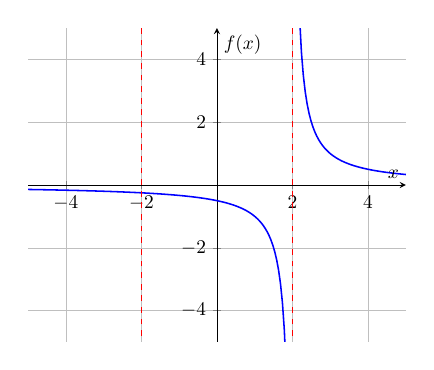
\begin{tikzpicture}[scale=0.7]
\begin{axis}[
    xmin=-5, xmax=5, ymin=-5, ymax=5,
    axis lines=center,
    samples=200,
    domain=-5:5,
    restrict y to domain=-10:10,
    xlabel={$x$}, ylabel={$f(x)$},
    xtick={-4,-2,0,2,4},
    ytick={-4,-2,0,2,4},
    grid=both,
    grid style={line width=.1pt, draw=gray!20},
    major grid style={line width=.2pt,draw=gray!50},
]
\addplot [blue, thick] {(x + 2)/(x^2 - 4)};
\draw [dashed, red] (axis cs:-2,-10) -- (axis cs:-2,10);
\draw [dashed, red] (axis cs:2,-10) -- (axis cs:2,10);
\end{axis}
\end{tikzpicture}
\end{center}

\subsubsection*{Horizontal Asymptotes}

Determined by the degrees of the numerator and denominator polynomials.

- **Degree of numerator \( < \) degree of denominator**:

  Horizontal asymptote at \( y = 0 \).

- **Degrees equal**:

  Horizontal asymptote at \( y = \dfrac{\text{leading coefficient of numerator}}{\text{leading coefficient of denominator}} \).

- **Degree of numerator \( > \) degree of denominator**:

  No horizontal asymptote; may have an oblique (slant) asymptote.

\textbf{Example}:

Find horizontal asymptote of \( f(x) = \dfrac{2x^2 + 3}{x^2 - x} \).

Degrees are equal (\( n = 2 \)), so:

\[
y = \dfrac{2}{1} = 2
\]

Horizontal asymptote at \( y = 2 \).

\textbf{Graph}:

\begin{center}
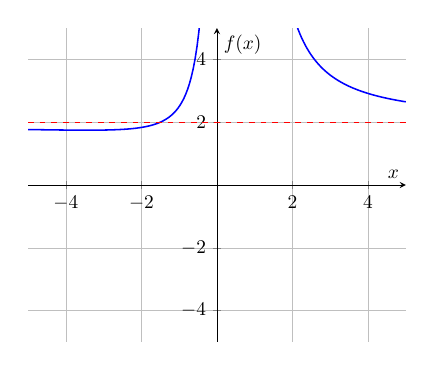
\begin{tikzpicture}[scale=0.7]
\begin{axis}[
    xmin=-5, xmax=5, ymin=-5, ymax=5,
    axis lines=center,
    samples=200,
    domain=-5:5,
    restrict y to domain=-10:10,
    xlabel={$x$}, ylabel={$f(x)$},
    xtick={-4,-2,0,2,4},
    ytick={-4,-2,0,2,4},
    grid=both,
    grid style={line width=.1pt, draw=gray!20},
    major grid style={line width=.2pt,draw=gray!50},
]
\addplot [blue, thick] {(2*x^2 + 3)/(x^2 - x)};
\draw [dashed, red] (axis cs:-5,2) -- (axis cs:5,2);
\end{axis}
\end{tikzpicture}
\end{center}

\subsection*{Identifying Cubic Graphs Based on Roots}

For a cubic polynomial \( f(x) = a(x - r_1)(x - r_2)(x - r_3) \):

- The graph crosses the \( x \)-axis at roots \( r_1, r_2, r_3 \).
- The behavior at each root depends on multiplicity.

\textbf{Example}:

Given \( f(x) = (x + 2)(x - 1)^2 \):

- Roots at \( x = -2 \) (multiplicity 1) and \( x = 1 \) (multiplicity 2).
- At \( x = -2 \), the graph crosses the \( x \)-axis.
- At \( x = 1 \), the graph touches and turns around (due to multiplicity 2).

\textbf{Graph}:

\begin{center}
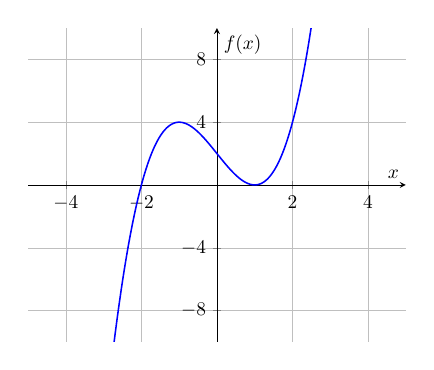
\begin{tikzpicture}[scale=0.7]
\begin{axis}[
    xmin=-5, xmax=5, ymin=-10, ymax=10,
    axis lines=center,
    samples=200,
    domain=-5:5,
    xlabel={$x$}, ylabel={$f(x)$},
    xtick={-4,-2,0,2,4},
    ytick={-8,-4,0,4,8},
    grid=both,
    grid style={line width=.1pt, draw=gray!20},
    major grid style={line width=.2pt,draw=gray!50},
]
\addplot [blue, thick] {(x + 2)*(x - 1)^2};
\end{axis}
\end{tikzpicture}
\end{center}

\end{multicols}

\end{document}
